\subsection{Session 4, Exercise 8}

\lineparagraph{Exercise}

Create a pushdown automaton for the language of proper parenthesisations.

\lineparagraph{Solution}

Idea: correct parenthesisation can be checked by counting from left to right: start with $0$ and add $+1$ for every $($ encountered and $-1$ for every $)$ encountered. The parenthesisation is correct if the sum never drops below $0$ during the calculation (too many $)$ in that case at that point) and at the end it equals to $0$. A simple PDA can be constructed to do exactly this calculation.


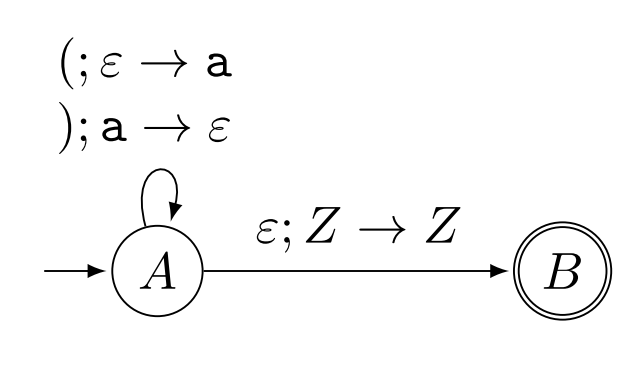
\includegraphics[width=0.4\linewidth]{04/4_8.png}

TODO Proof